\PassOptionsToPackage{table}{xcolor}

\documentclass[sigconf]{acmart}

\AtBeginDocument{%
  \providecommand\BibTeX{{%
    \normalfont B\kern-0.5em{\scshape i\kern-0.25em b}\kern-0.8em\TeX}}}

\copyrightyear{2020} 
\acmYear{2020} 
\setcopyright{rightsretained} 
\acmConference[Web3D '20]{The 25th International Conference on 3D Web Technology}{November 9--13, 2020}{Virtual Event, Republic of Korea}
\acmBooktitle{The 25th International Conference on 3D Web Technology (Web3D '20), November 9--13, 2020, Virtual Event, Republic of Korea}
\acmDOI{10.1145/3424616.3424730}
\acmISBN{978-1-4503-8169-7/20/11}

\acmSubmissionID{37}

\citestyle{acmauthoryear}

\usepackage{booktabs}
\usepackage{tabularx}
\usepackage{csquotes}
\usepackage{numprint}

\usepackage{tikz}
\usetikzlibrary{calc,positioning,spy}

\usepackage{eso-pic}
\AddToShipoutPictureFG{\AtPageLowerLeft{\put(\LenToUnit{0.5\paperwidth},\LenToUnit{6mm}){\makebox[0pt][c]{\fontsize{6.5}{8}\selectfont\color{gray}Author's revised version (2026-11-08). Version of record: https://doi.org/10.1145/3424616.3424730}}}}

\begin{document}

\title{A Framework for Interactive Exploration of Clusters in Massive Data Using 3D Scatter Plots and WebGL}

\author{Lukas Wagner}
\orcid{0000-0002-5934-3310}
\affiliation{%
  \institution{Hasso Plattner Institute,\\University of Potsdam, Germany}
}
\email{lukas.wagner@hpi.de}

\author{Daniel Limberger}
\orcid{0000-0002-9111-4809}
\affiliation{%
  \institution{Hasso Plattner Institute,\\University of Potsdam, Germany}
}
\email{daniel.limberger@hpi.de}

\author{Willy Scheibel}
\orcid{0000-0002-7885-9857}
\affiliation{%
  \institution{Hasso Plattner Institute,\\University of Potsdam, Germany}
}
\email{willy.scheibel@hpi.de}

\author{Matthias Trapp}
\orcid{0000-0003-3861-5759}
\affiliation{%
  \institution{Hasso Plattner Institute,\\University of Potsdam, Germany}
}
\email{matthias.trapp@hpi.de}

\author{J{\"u}rgen D{\"o}llner}
\orcid{0000-0002-8981-8583}
\affiliation{%
  \institution{Hasso Plattner Institute,\\University of Potsdam, Germany}
}
\email{juergen.doellner@hpi.de}

\renewcommand{\shortauthors}{Wagner et al.}

\begin{abstract}
This paper presents a rendering framework for the visualization of massive point datasets on the web.
It includes highly interactive point rendering, cluster visualization, basic interaction methods, and importance-based labeling, while being available for both mobile and desktop browsers.
The rendering style is customizable, as shown in Figure~\ref{fig:teaser}.
Our evaluation indicates that the framework facilitates interactive visualization of tens of millions of raw data points even without dynamic filtering or aggregation.
\end{abstract}

\keywords{WebGL, scatter plot, massive data, cluster visualization, framework}

\begin{teaserfigure}%
    \centering
    \begin{tikzpicture}[spy using outlines={white, rectangle, magnification=4.0, size=52, connect spies, every spy on node/.append style={thin}},inner sep=0pt, outer sep=0pt]
        \node[anchor=west](left) at (-0.5\linewidth,0) {%
            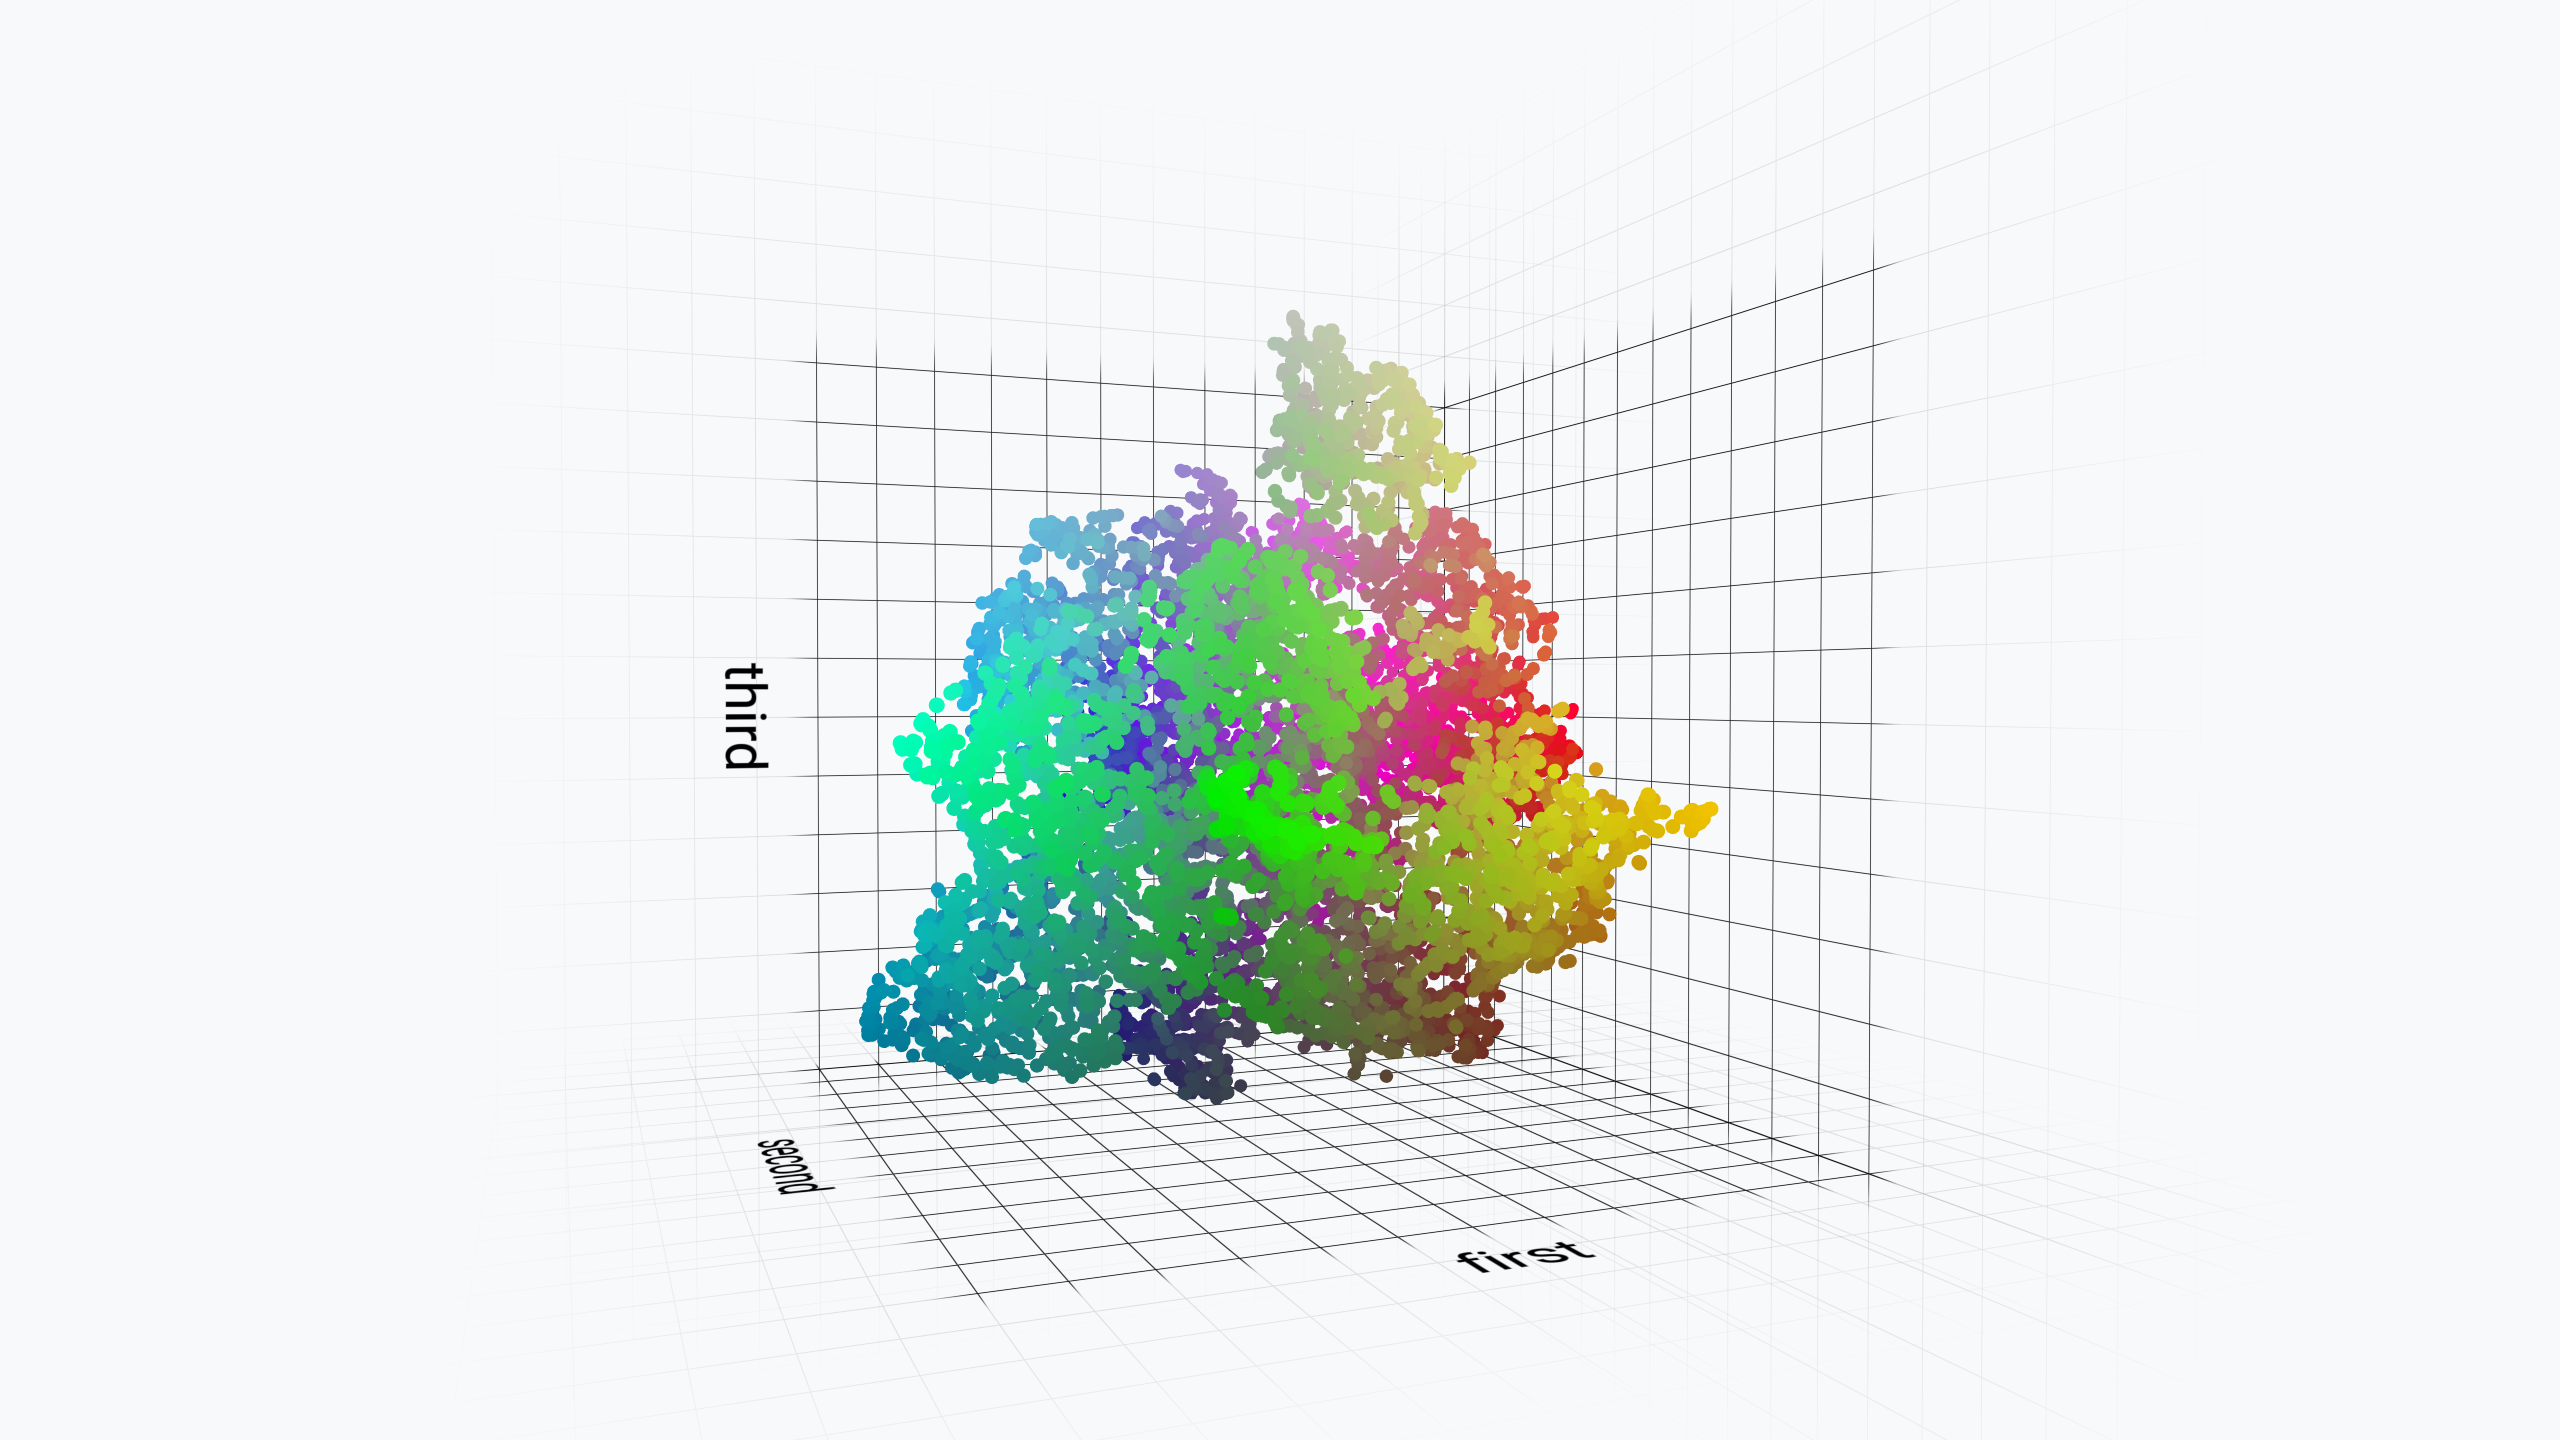
\includegraphics[trim=300 100 300 200, clip, width=0.32\textwidth]{tm_teaser2.png}};%
        \spy [black] on ($(left.center)+(0.3, -0.1)$) in node at ($(-1.8, 0.65)+(left.center)$);
        \node[anchor=center, inner sep=0pt, outer sep=0pt](middle) at (0,0) {%
            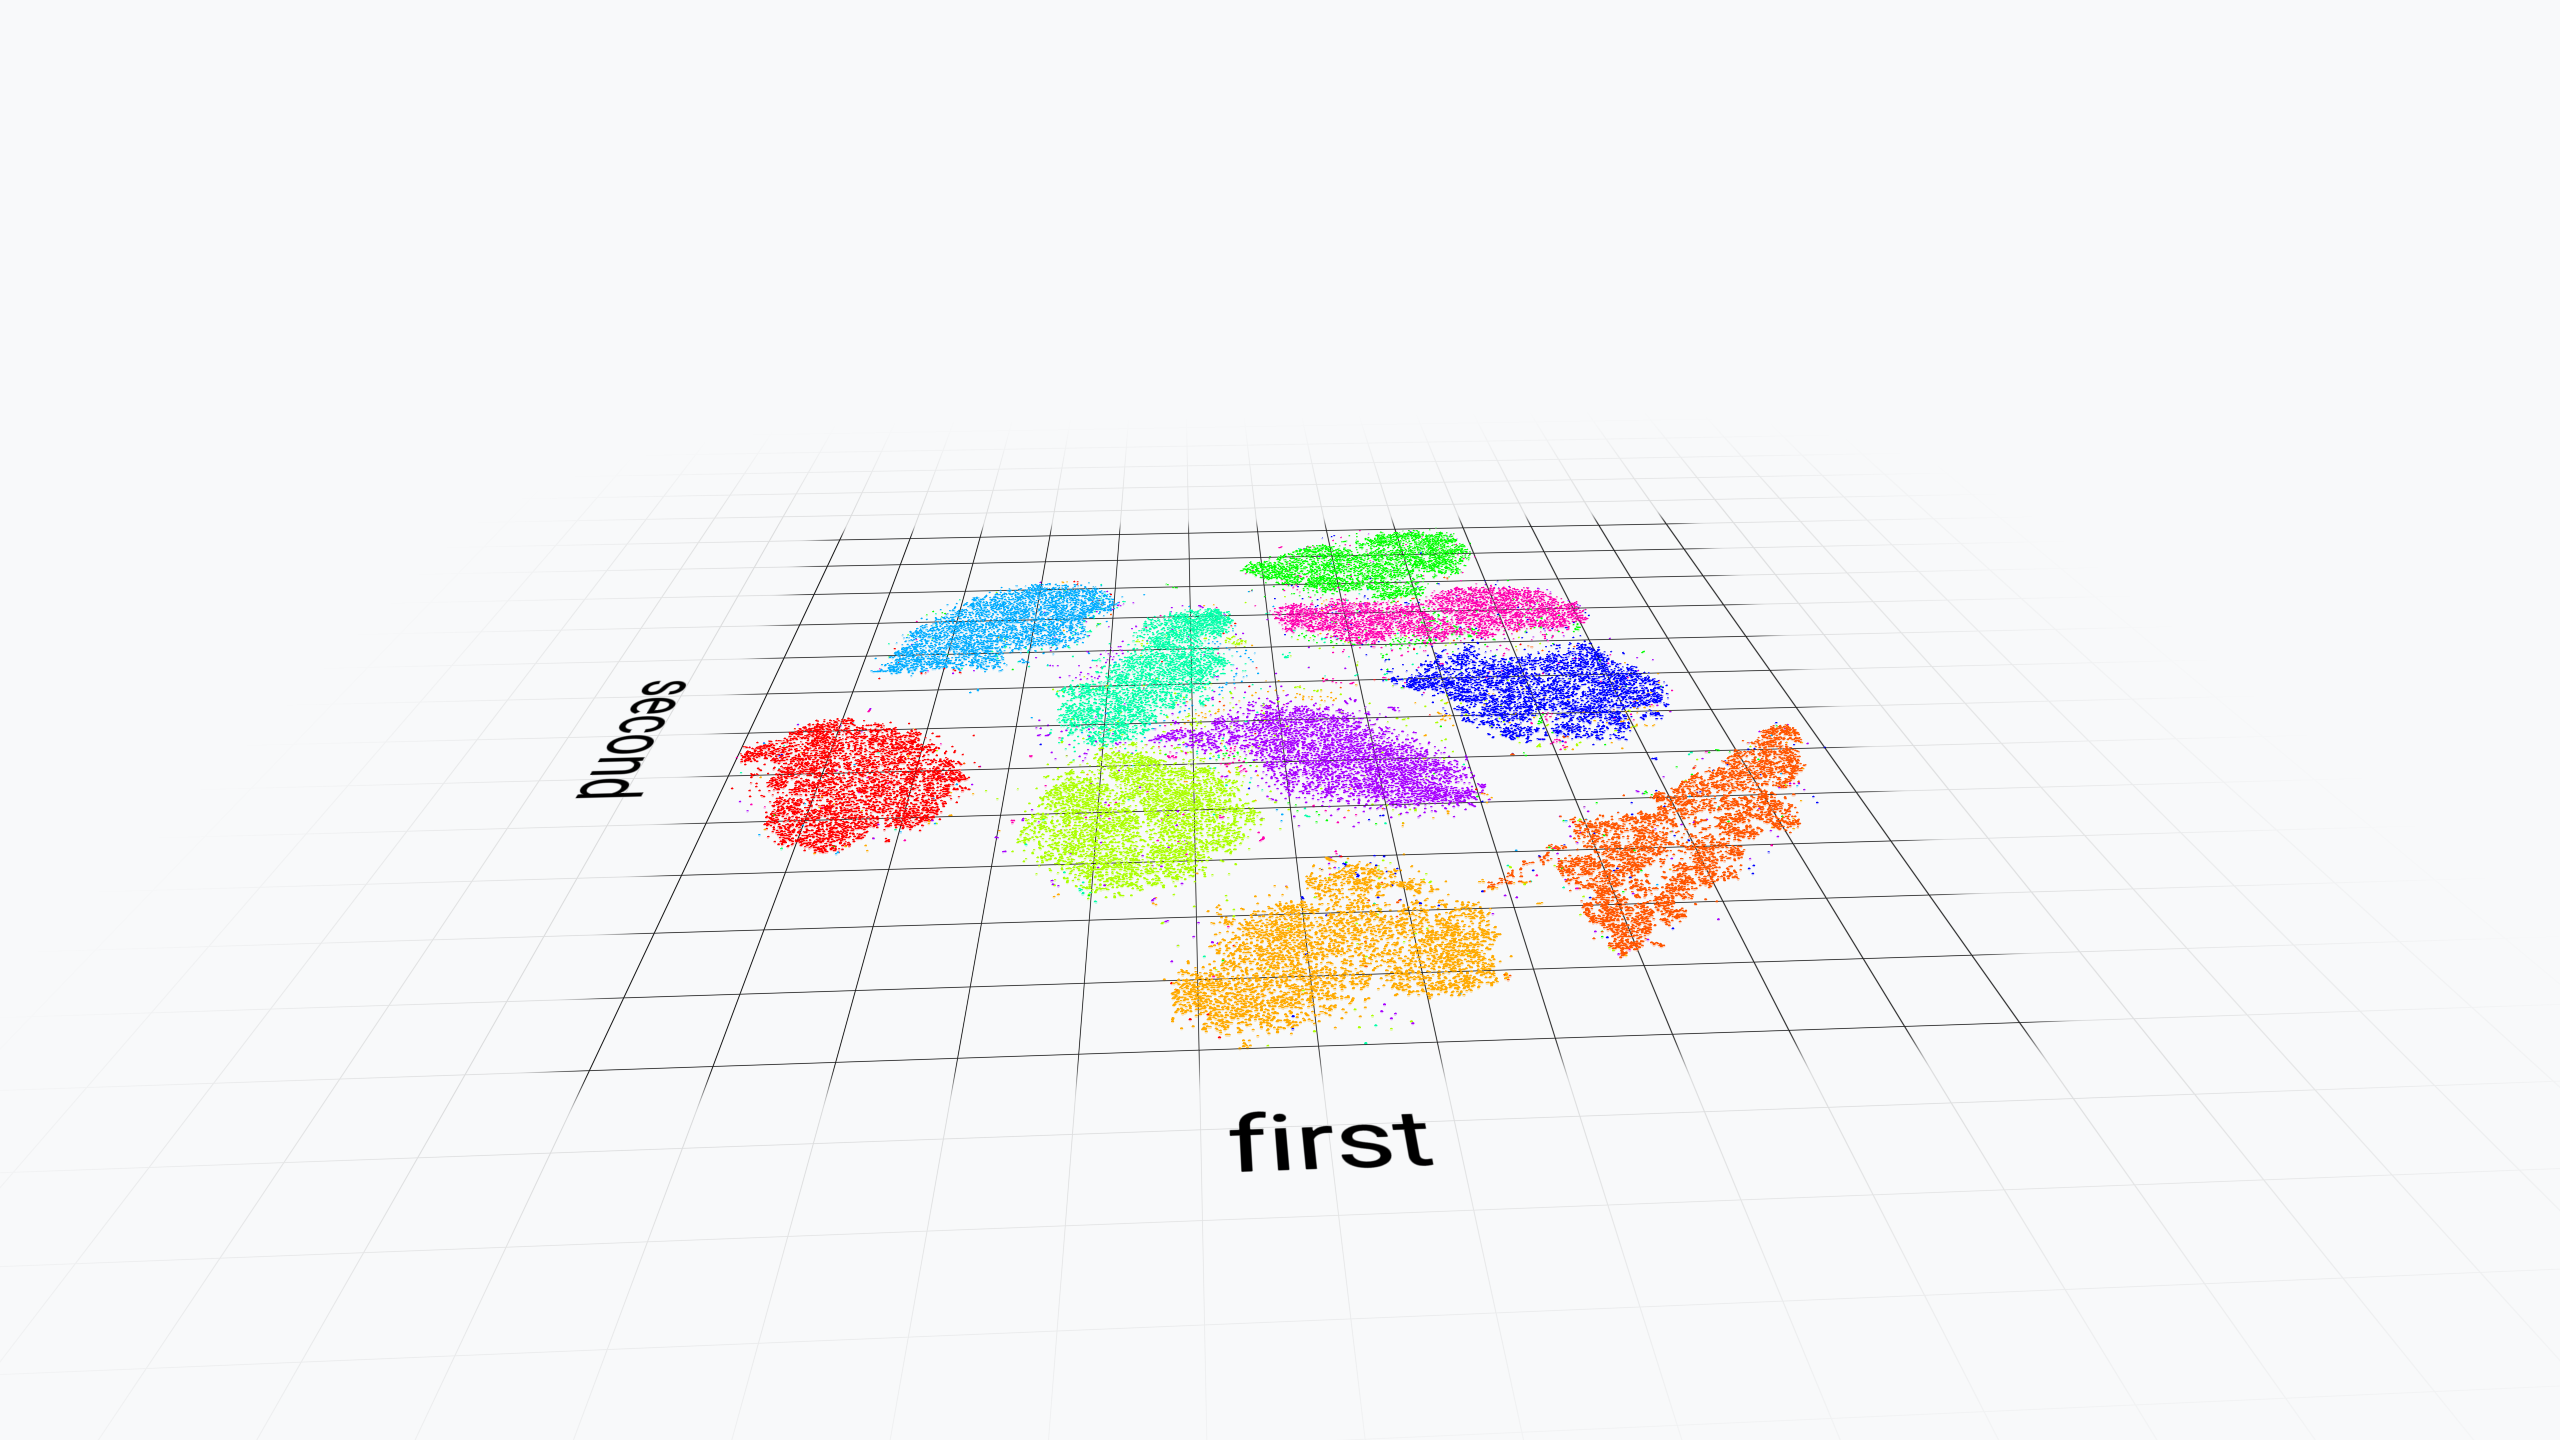
\includegraphics[trim=300 150 300 150, clip, width=0.32\textwidth]{handwriting2.png}};%
        \spy [black] on ($(middle)+(0.7, +0.2)$) in node at ($(-1.8, 0.65)+(middle.center)$);
        \node[anchor=east, inner sep=0pt, outer sep=0pt](right) at (0.5\linewidth, 0) {%
            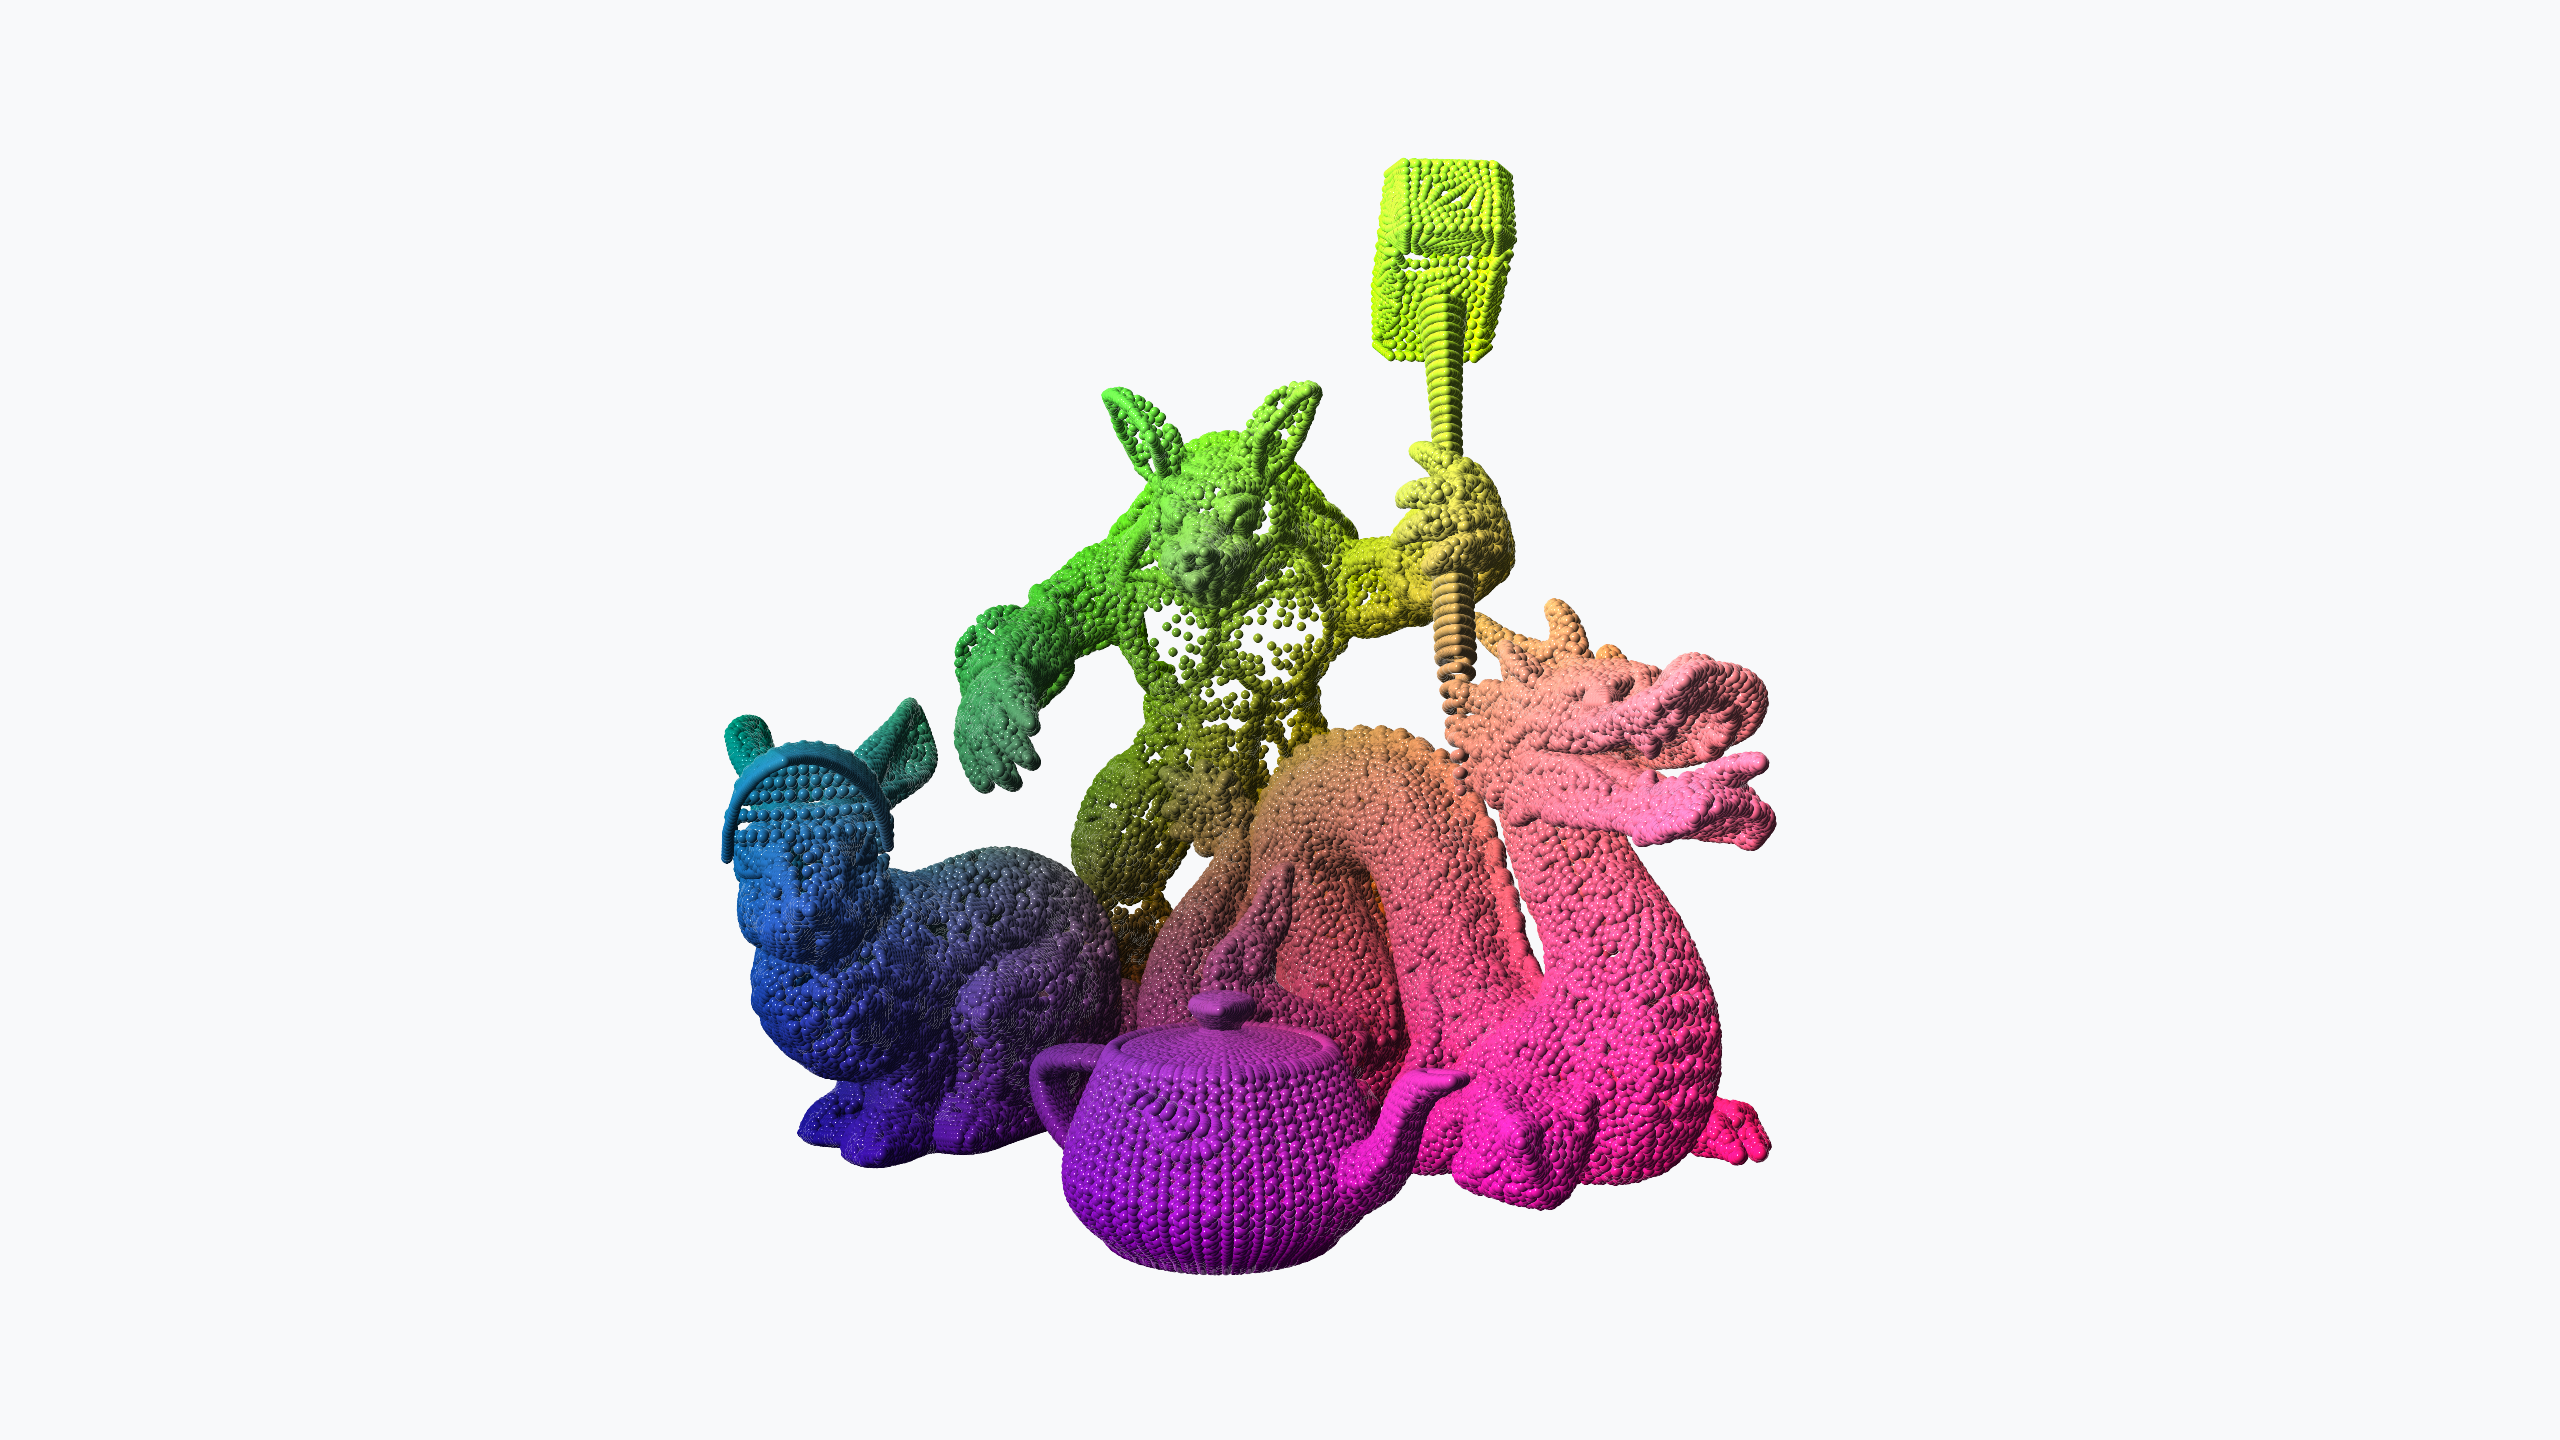
\includegraphics[trim=300 150 300 150, clip, width=0.32\textwidth]{khronos_white.png}};%
        \spy [black] on ($(right.center)+(1.3, +0.0)$) in node at ($(-1.8, 0.65)+(right.center)$);
    \end{tikzpicture}
    \vspace{-0.6cm}
    \caption{Various datasets visualized with our rendering framework. From left to right: \numprint{11000} documents, arranged using dimension reduction based on topic similarities; MNIST handwritten digits dataset, arranged using t-SNE dimension reduction; different theme (using Phong shading and larger point diameter) showing \numprint{140000} vertices of the Khronos figures.}
    \label{fig:teaser}
\end{teaserfigure}

\maketitle

\section{Introduction}

With the advance of computational capabilities, the amount of available data grows steadily, to previously unfathomable ranges~\cite{ridiculousstoragesilos}. 
The need for improved processing methods brought about new research topics such as machine learning and big data. 
While this allows utilizing the data, human comprehension remains a challenge. 
It is often not feasible for a human observer to visualize and understand these huge and often high-dimensional datasets.
This has prompted extensive research in Big Data visualization~\cite{visExpLargeData,interactivebigdatavis,po2020linked}.
End-user facing applications typically used for plotting data, such as Microsoft Excel, simply cannot cope with this amount of data. 
Even custom-built visualizations using plotting frameworks, e.g., the commonly used D3 library, fall short when trying to draw huge datasets.
The capabilities of D3, for example, are limited by the web browsers' SVG rendering engine. 
In the past, it was necessary to harness the power of low-level APIs such as OpenGL to achieve the required performance. 
With the advance of technologies such as WebGL and the upcoming WebGPU standard, it has become feasible to create complex web-based visualizations. 
This allows for an OS- and (mostly) browser-agnostic implementation, resulting in very lax requirements on the end users' hardware.
Following this shift, research topics, which have historically only been feasible with a low-level approach, such as point clouds, have seen successful web-based implementations. Two notable examples are Potree\footnote{\href{http://potree.org/}{potree.org}}, a specialized point cloud viewer, and CesiumJS\footnote{\href{https://cesium.com/cesiumjs/}{cesium.com/cesiumjs}}, a more generalized geospatial toolkit~\cite{potree,cesiumpoints}.
Point clouds require millions of data points to be rendered.
While these points do not provide any meaning individually, they can illustrate very complex scenes.
This distinguishes point clouds from a regular plotting approach, where every point carries data.

In order to allow for an easier overview of the dataset, as well as to approach the occlusion problem \cite{occlusion}, we analyze the point cloud using clustering algorithms such as $\alpha$-shapes \cite{alphaclusters}.
Reducing millions of points to significantly fewer clusters (typically in the magnitude of~10) gives a high-level view of the data~\cite{multidimclusters}.
Additionally, the clusters can be used to reduce concealment issues.
By representing multiple points with a single object of less extent, more of the dataset is visible at once, while still providing a meaningful representation.
In combination with a multi-level clustering approach, the dataset can be explored both on a high level and in detail.
Picking and labeling techniques can be used to quickly spot relevant clusters.
After focusing on a cluster, the user can increase its level-of-detail to view subclusters and individual data points.

\paragraph{Contributions}
We present a new web-based rendering framework for visualizing and exploring massive datasets, capable of interactively visualizing tens of millions of data points. In order to facilitate understanding, we utilize a dual rendering approach to both give a high-level overview of the dataset, as well as allow low-level interaction with single datapoints simultaneously.

\section{Rendering Approach}

In order to render massive datasets, they first have to be loaded and possibly preprocessed by the CPU. As this task can take a while, depending on size and format of the input file, we use a streaming approach. While the data source is being read, any chunks of datapoints that have been read already are immediately made available for rendering by handing the data over to the GPU. This allows the user to get a quick preview of the dataset without waiting for the whole source to be loaded. Additionally, this allows us to support nonfinite data sources, such as live sensors producing an endless stream of data.

For rendering the individual data points, we utilize instanced rendering.
Instead of creating an individual geometry for each point, a shared geometry is reused.
The geometry is then adjusted for each data point by passing along per-point data.
This technique significantly improves rendering performance and allows for custom shapes of varying complexity for multi-variate data mapping.

Since one goal of our visualization is to gain a high-level understanding of the dataset, we use clustering and dimension reduction techniques to group the data points.
These subsets allow for a multi-level rendering approach, where the surface of a set is used as a mesh, replacing any points contained in the set.
Thus, the underlying dataset could contain an arbitrary amount of points, as only the subsets currently in focus are rendered in high detail, while the remaining subsets are replaced with the high-level representation.
The user can then control the clusters' level of detail either indirectly through the camera position or directly by interacting with the clusters.
With this multi-level approach, the user can quickly gain an overview of the overall structure of the dataset as well as retrieve selective, per-point information.

\section{Implementation}

As noted in the introduction, we chose a web-based implementation to increase portability and simplify the user experience. Thus, we were limited to WebGL~2.
We chose webgl-operate\footnote{\href{https://webgl-operate.org/}{webgl-operate.org}} as the rendering framework.
In order to speed up loading and processing a dataset, we utilize threads to harness available CPU power.
When loading the data, we use a streaming interface to support both normal files, as well as data sent by a server using a stream.
The main thread receives the input in chunks.
These are handed over to worker threads for parsing, which arrange the data into columns, each representing one attribute.
By handling the input in chunks, any available data can be sent to the GPU immediately, enabling rendering of intermediate results.
The data is managed without any optimization structure such as an octree. While this would allow for handling of even bigger datasets, the current approach already allows rendering millions of points interactively, as seen in Table~\ref{tab:eval}.

\begin{table}[b]
    \renewcommand{\arraystretch}{0.95}
	\centering
	\small
	\noindent
	\caption{Frames per second for different amounts of data measured on a low-, mid-, and high-end GPU in Chrome 84.}%
	\vspace{-0.75\baselineskip}
	\label{tab:eval}
	\begin{tabularx}{\linewidth}{X|rrrrr}
		\toprule
		\hiderowcolors
		\textbf{Test System} & \multicolumn{5}{c}{\textbf{Number of Points}} \\
		in 1920$\times$1080px &\
		$1\times10^6$ &\
		$5\times10^6$ &\
		$1\times10^7$ &\
		$5\times10^7$ &\
		$1\times10^8$ \\
		\midrule
		\showrowcolors
		Intel UHD 630   &  26.8 &  18.6 &  10.8 &   2.6 &   1.4 \\
	    Nvidia GTX 1650 & 196.6 &  65.2 &  38.0 &   8.9 &   4.6 \\
		Nvidia GTX 1080 & 474.6 & 154.3 &  81.2 &  17.6 &   9.0 \\
		\bottomrule
	\end{tabularx}
\end{table}

\section{Conclusion}

We presented a new rendering framework for visualizing and exploring massive datasets. Using a highly optimized WebGL-based implementation, we can visualize tens of millions of data points interactively.
In order to facilitate understanding, we utilize a dual rendering approach to both give a high-level overview of the dataset, as well as allow low-level interaction with single datapoints.

\bibliographystyle{ACM-Reference-Format}
\bibliography{references}

\end{document}
\endinput
